% RESULTADOS-------------------------------------------------------------------

\chapter{APRESENTAÇÃO E ANÁLISE DE RESULTADOS}

Aqui serão detalhados os resultados obtidos com o funcionamento do circuito desenvolvido integrado a um forno microondas convencional da marca Panasonic. Nesta capítulo será descrito o funcionamento prático do circuito, expondo o resultado da medições de parâmetros que avaliam a performance e fazendo comparações com os parâmetros do circuito ferrorressonante original do forno microondas utilizado.


\section{Sistema em Funcionamento}
A placa original do aparelho foi removida e trocada pela placa desenvolvida, ligando-se todos os fios que conectam o circuito projetado à rede e ao magnetron maneira similar à original. Para acionar o circuito, foi utilizada a interface já presente no forno, configurando o nível percentual de potência e o tempo de cozimento de acordo com os experimentos realizados. Para testar o funcionamento, a equipe acionou o circuito em diferentes configurações de potência, medindo-se as formas de onda em diferentes pontos para demonstrar o funcionamento prático do sistema. As subseções a seguir irão descrever este funcionamento.

\subsection{Corrente e potência}
A fim de se verificar o funcionamento correto do circuito montado, as formas da corrente no \textit{shunt} foram verificadas com um osciloscópio digital. A figura abaixo mostra o resultado obtido com o circuito operando em potência máxima:

\begin{figure}[H]
    \centering
    \caption{Formas de onda da tensão e corrente}
    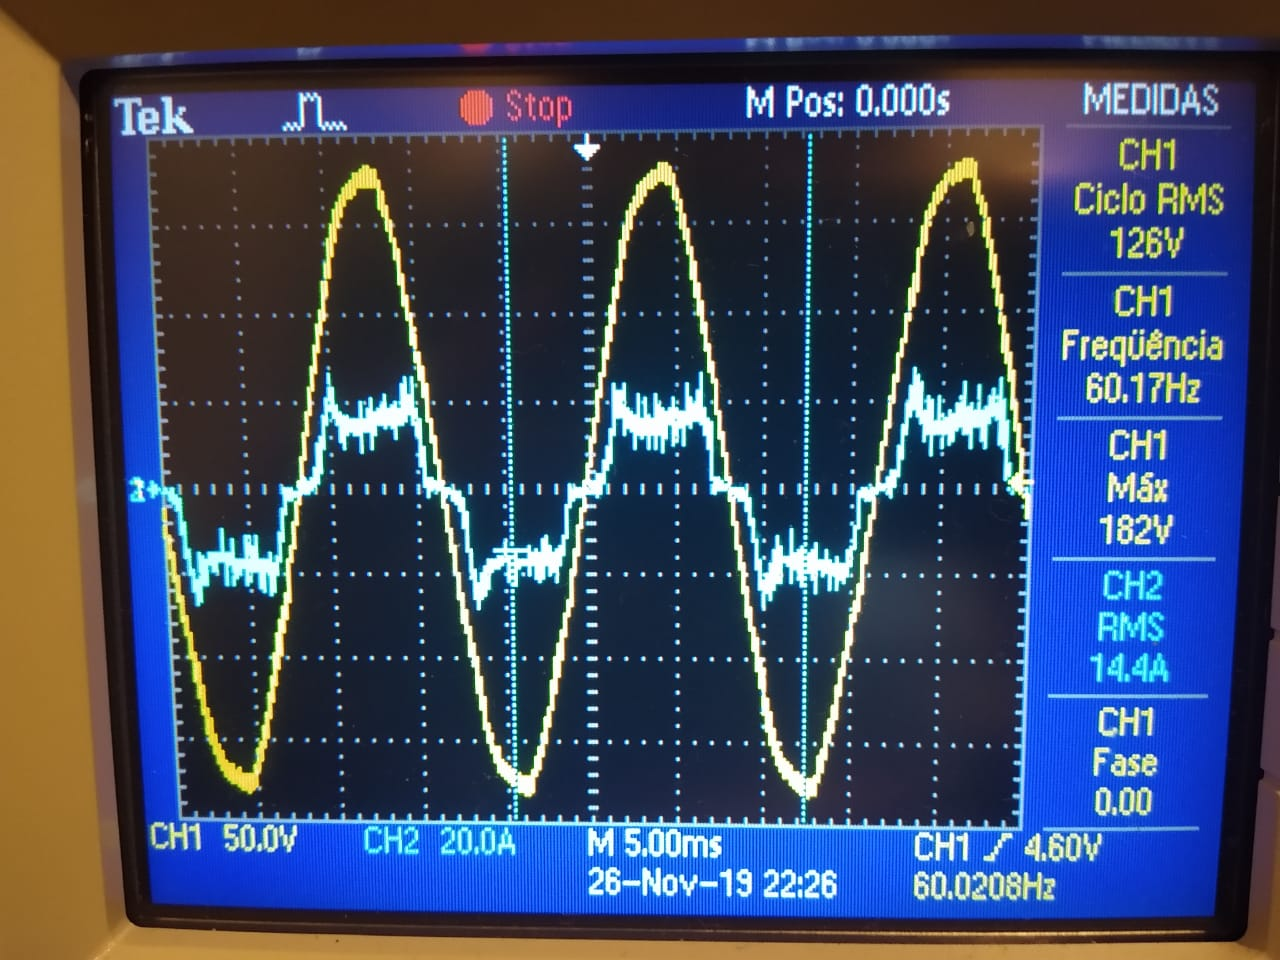
\includegraphics[width=0.8\textwidth]{./dados/figuras/onda_corrente}
    \fonte{Autoria própria (2019)}
    \label{fig:figura-onda_corrente}
\end{figure}

Na figura, a forma de onda azul (canal 2) é a corrente no \textit{shunt}, enquanto a outra forma de onda, em amarelo (canal 1) é a tensão da rede. Como pode-se observar, o valor da corrente é muito elevado, atingindo um valor RMS de 14,4 A.  A medida que o nível de potência varia, maior o valor RMS da corrente e mais a forma de onda tende a suavizar a curvatura que tem em direção ao eixo horizontal. A forma de onda segue o mesmo ciclo que o sinal da tensão da rede, tendo um \textit{ripple} extremamente elevado. Este \textit{ripple} nada mais é que a consequência do forte ruído gerado pelas emissões do magnetron. Saleinta-se que o ambiente do experimento não era controlado, e que o chassi metálico do forno não estava completamente fechado, o que contribui também para distorções na forma de onda.

Para medir a potência consumida pelo circuito, foi utilizado um medidor de energia elétrica comercial portátil, no qual se conecta a alimentação do forno, enquanto a alimentação do medidor é ligada na tomada no lugar do aparelho. A figura abaixo mostra a leitura obtida no mesmo experimento:

\begin{figure}[H]
    \centering
    \caption{Leitura de potência obtida}
    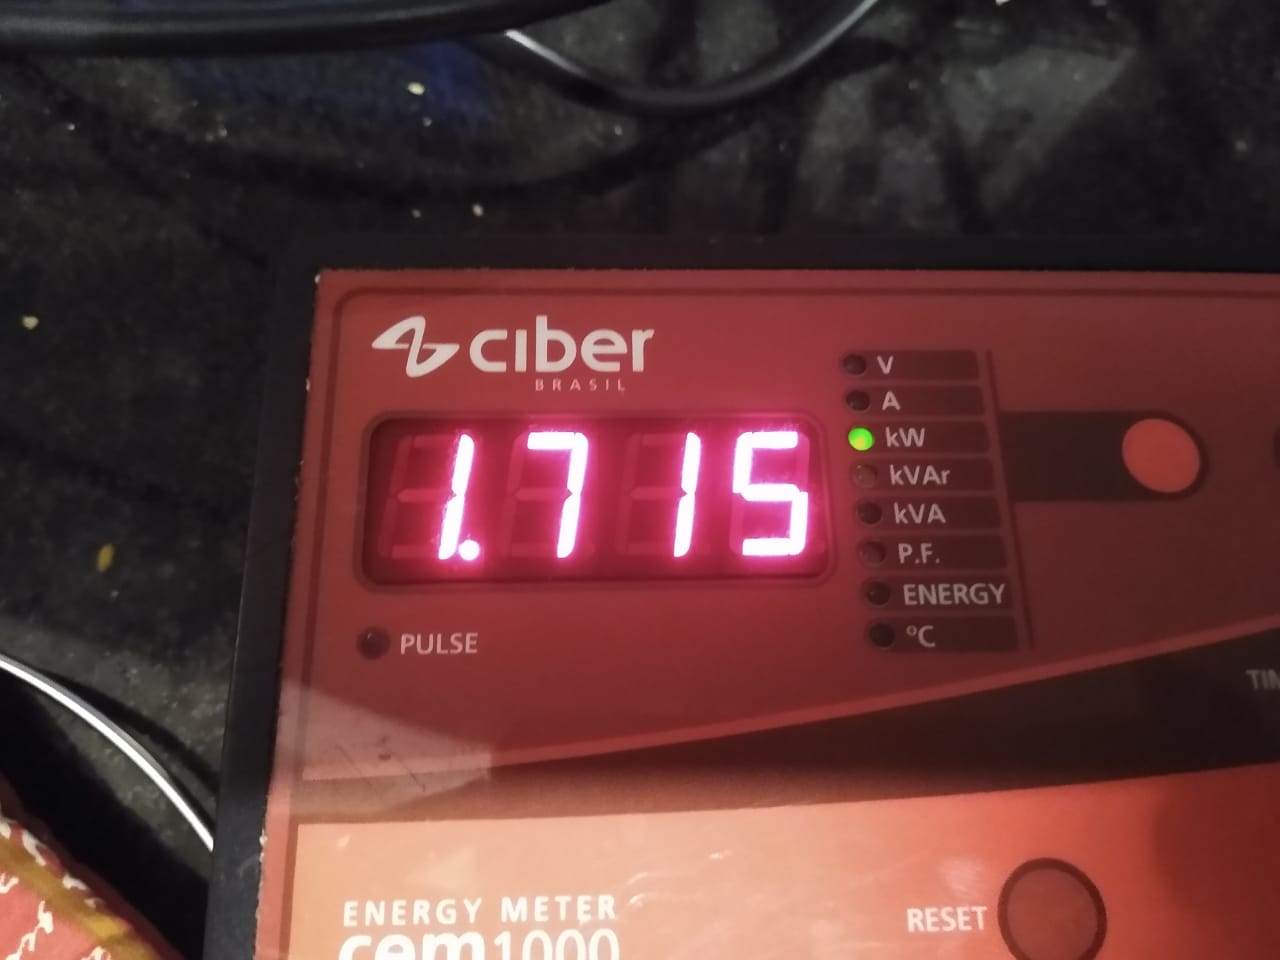
\includegraphics[width=0.8\textwidth]{./dados/figuras/medida_potencia_full}
    \fonte{Autoria própria (2019)}
    \label{fig:figura-medida_potencia_full}
\end{figure}

A leitura obtida, como pode-se notar, é de 1715 W. Salienta-se que esta potência corresponde a soma da potência da alimentação do magnetron, da lâmpada e do motor do prato giratório dentro do forno. Pelo manual do aparelho, tem-se que a potência aproximada utilizada pelo motor e pela lâmpada é de aproximadamente 100 W. Ao calcular-se a potência teórica pelos valores RMS medidos na figura \ref{fig:figura-onda_corrente}, obtém-se 1814 W. Para este experimento não foi feita uma calibração com os devidos equipamentos, e portanto não se tem uma precisão elevada para as medições. Outro fator que influencia na precisão, é o elevado ruído de alta frequência detectado na forma de onda da corrente, que também deteriora a qualidade da medição. Para este experimento, a equipe configurou o algoritmo de controle com uma potência máxima de 1600 W, logo com potência máxima utilizada pelo forno de cerca de 1700 W. Devido aos fatores prejudiciais à precisão do experimento, citados anteriormente, o valor real da potência atingida pode sofrer uma pequena alteração percentual. De forma geral, tem-se que a potência obtida pelo experimento está dentro do que foi esperado pela equipe, visto que em ambas as medições o valor medido não ultrapassou os 10\% de tolerância estabelecido.

\subsection{Chaveamento dos IGBTs}
O chaveamento dos IGBTs é o que faz efetivamente o controle da potência do magnetron, bloqueando o sinal de tensão no primário quando os dispositivos são colocados em \textit{off}. Para realizar o controle, a planta desenvolvida controla dois parâmetros do sinal da porta do dispositivo: frequência e ciclo de trabalho. As figuras abaixo mostram o circuito operando em três configurações. Em amarelo, no canal 1 é mostrado o sinal do IGBT. Em azul, no canal 2, é mostrada a tensão de barramento, enquanto no canal 3, em rosa, mostra-se o sinal que vai para o conversor AD de tensão:

\begin{figure}[H]
    \centering
    \caption{Formas de onda: caso 1}
    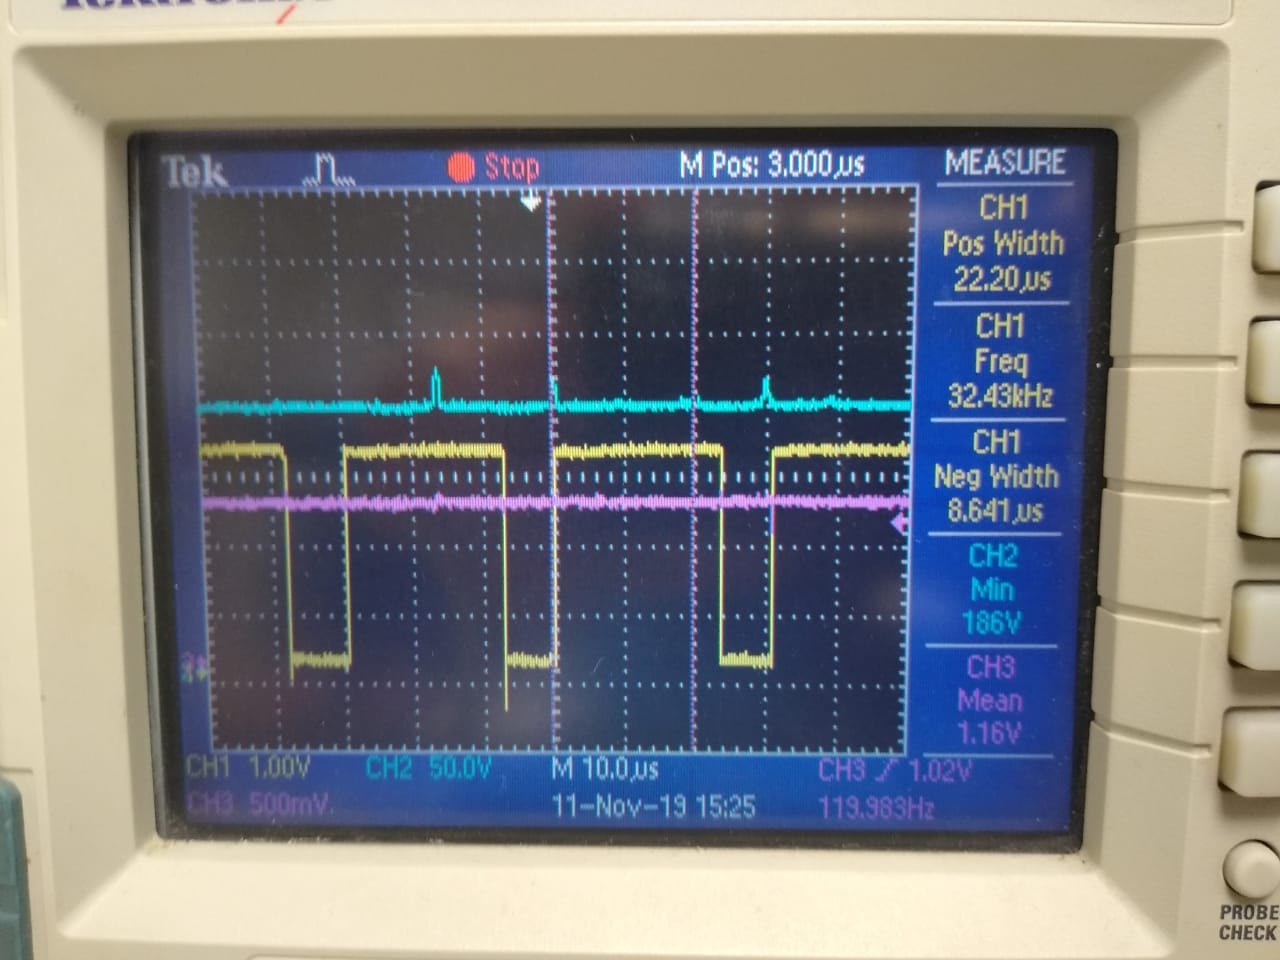
\includegraphics[width=0.8\textwidth]{./dados/figuras/onda_controller_1}
    \fonte{Autoria própria (2019)}
    \label{fig:figura-onda_controller_1}
\end{figure}

\begin{figure}[H]
    \centering
    \caption{Formas de onda: caso 2}
    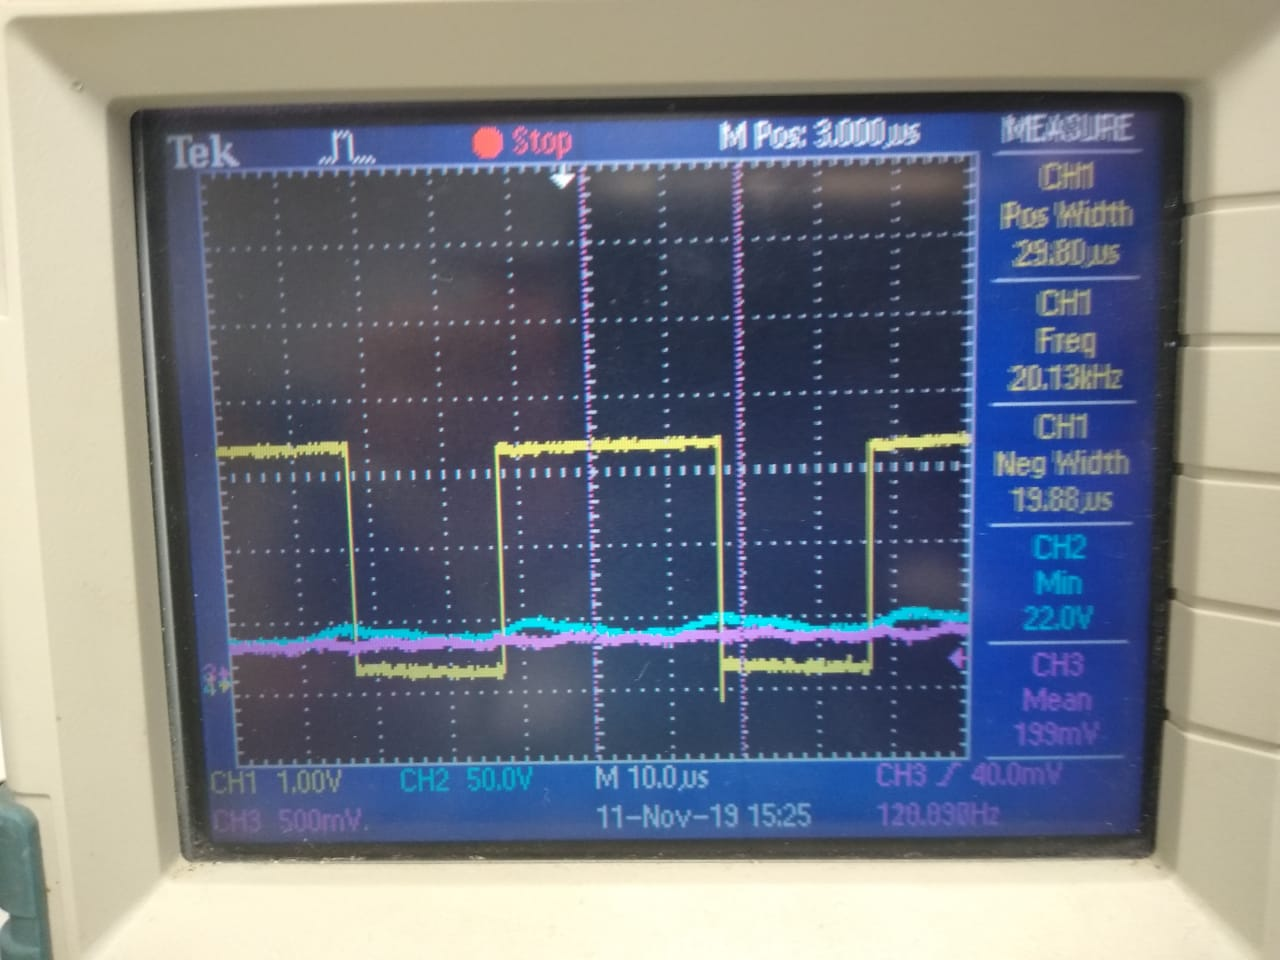
\includegraphics[width=0.8\textwidth]{./dados/figuras/onda_controller_2}
    \fonte{Autoria própria (2019)}
    \label{fig:figura-onda_controller_2}
\end{figure}

\begin{figure}[H]
    \centering
    \caption{Formas de onda: caso 3}
    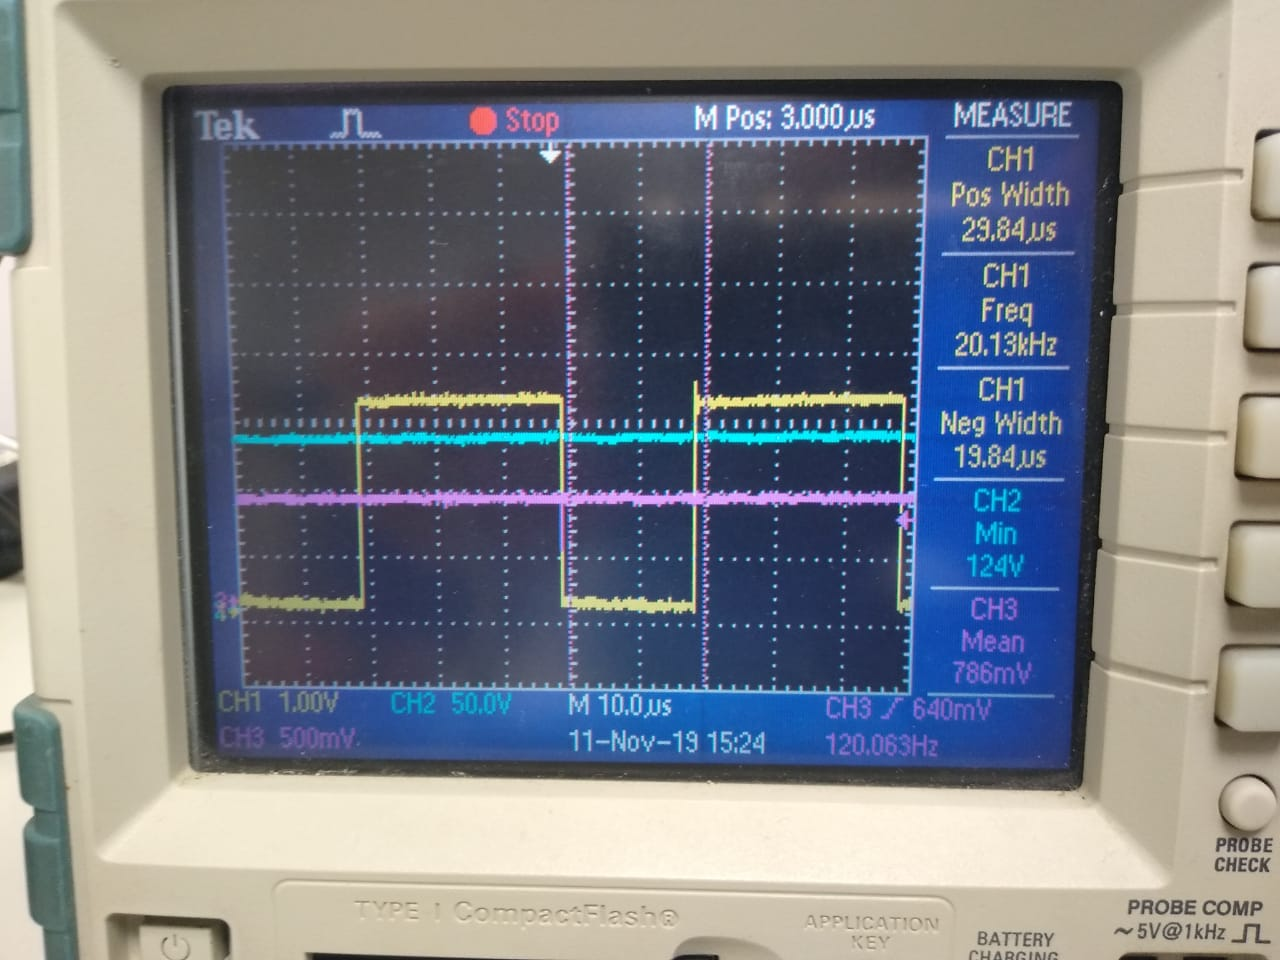
\includegraphics[width=0.8\textwidth]{./dados/figuras/onda_controller_3}
    \fonte{Autoria própria (2019)}
    \label{fig:figura-onda_controller_3}
\end{figure}

Nas figuras mostradas, tem-se três situações: 
\bigskip
\begin{itemize}
    \item Ciclo de trabalho 70\%, frequência de 32 kHz e tensão do ADC de 1,16 V;
    \item Ciclo de trabalho 60\%, frequência de 20 kHz e tensão do ADC de 199 mV;
    \item Ciclo de trabalho 60\%, frequência de 20 kHz e tensão do ADC de 786 mV.
\end{itemize}
\bigskip

Cada situação mostra uma diferente decisão tomada pelo \textit{firmware} desenvolvido. A planta desenvolvida, através da realimentação de corrente e cálculo da potência com a medição do conversor AD, determinou o valor do ciclo e trabalho e frequência utilizada no chaveamento para regular a potência no valor estabelecido. Um maior ciclo de trabalho não implica necessariamente numa maior potência, visto que a frequência do sinal exerce um papel fundamental na determinação da potência de saída, dadas às características do circuito.

\subsection{Sinais de controle e status}
Os sinal de controle determina a potência solicitada pelo magnetron e o sinal de status verifica se o sistema está operando corretamente. A figura abaixo mostra as formas de onda medidas destes dois sinais operando com potência máxima:

\begin{figure}[H]
    \centering
    \caption{Formas de onda dos sinais de comunicação}
    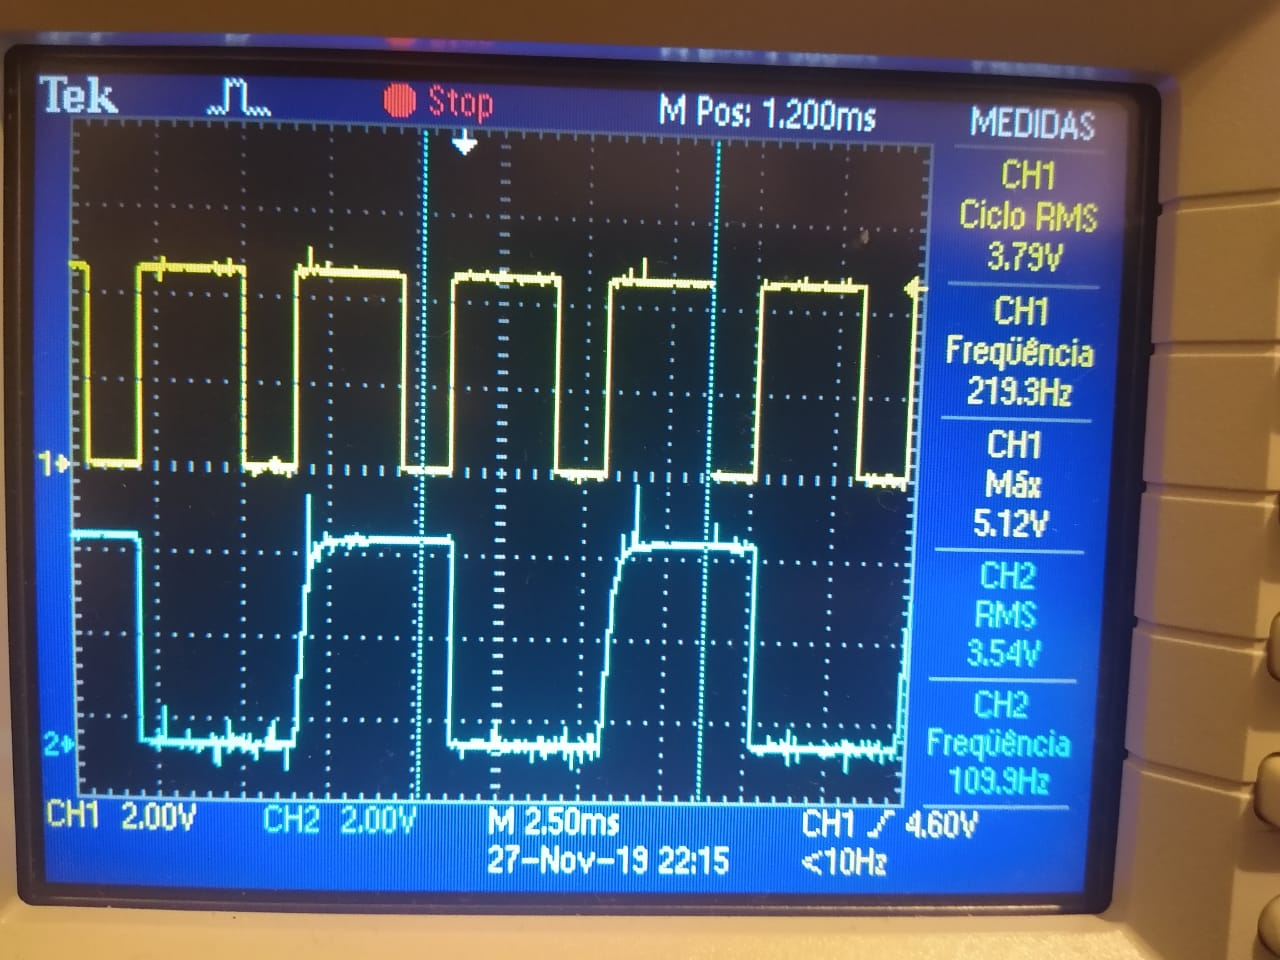
\includegraphics[width=0.8\textwidth]{./dados/figuras/onda_comm}
    \fonte{Autoria própria (2019)}
    \label{fig:figura-onda_comm}
\end{figure}

Em amarelo, no canal 1, é mostrado o sinal de controle. O ciclo de trabalho de 75\% representa a solicitação de potência máxima. Caso a potência solicitada diminua, o ciclo de trabalho também irá diminuir, e abaixo de um ciclo de 50\%, a forma de onda deixa de ser continua, ficando um determinado intervalo de tempo com 0 V. Quanto ao sinal de status, nota-se que o mesmo é uma onda quadrada contínua, com ciclo de trabalho fixado em 50\%, sendo sincronizado com a forma de onda do sinal de controle. Portanto, de acordo com o projeto do algoritmo para a interface de comunicação, descrito na seção \ref{sec:plant}, pode-se considerar que o resultado obtido está de acordo com o comportamento previsto.


\section{Medições de parâmetros}
\label{sec:mesaures}
Para comparar o desempenho do circuito desenvolvido com uma fonte ferrorressonante tradicional, foram medidos três parâmetros essenciais para se possibilitar uma discussão válida sobre o tema: eficiência, fator de potência e dimensões físicas, incluindo massa, altura, largura e comprimento. 

\subsection{Eficiência}
A eficiência do forno microondas pode ser avaliada de forma geral como a performance do circuito de alimentação do magnetron. Este parâmetro pode ser obtido fazendo-se uma relação entre o calor absorvido pelo líquido dentro na câmara de cozimento do forno e a energia elétrica consumida pelo circuito.
Para avaliar a performance, a equipe se baseou em um experimento que é utilizado pelo INMETRO para determinar a eficiência de fornos microondas, o qual está detalhado em \citeonline{Inmetro}. O experimento consiste em esquentar 1 litro de água em um determinado tempo. A realização do experimento não seguiu totalmente os critérios estipulados pelo INMETRO, visto que a experiência não foi feita em ambiente controlado e o recipiente utilizado não é possui as dimensões, peso e material recomendados. A água usada no teste estava armazenada em um recipiente aberto de vidro, o qual tem massa de 600g. Antes da realização da experiência, a equipe aqueceu o recipiente vazio para determinar se o mesmo aquecia de forma significativa sem a presença de água, a fim de verificar se o recipiente poderia interferir nas medições. Inicialmente o recipiente se encontrava em temperatura ambiente de 20 ºC. Após colocá-lo no microondas por 60 segundos, o recipiente apresentou temperatura de 22 ºC. Logo a variação foi de 2 ºC, a qual não acarreta em impactos significativos na precisão das medidas.
Inicialmente mediu-se a temperatura da água no recipiente, utilizando-se um termopar industrial comum. Feito isso, o recipiente foi colocado no forno e acionado em potência máxima durante 65 segundos. Então, retirou-se a o recipiente do aparelho e com o termopar mediu-se a temperatura. Através das fórmulas descritas em \citeonline{Inmetro}, mediu-se a eficiência do circuito. No total, foram realizados dois experimentos, cada qual possuindo uma temperatura da água distinta. O tempo de aquecimento não é o tempo de cozimento selecionado no teclado do forno pois o magnetron utilizado leva cerca de 4 segundos para ter seu filamento aquecido e começar a emitir radiação. Seja $T_i$ a temperatura inicial, $T_f$ a temperatura final, $T_\mathrm{amb}$ a temperatura ambiente, $t_\mathrm{total}$ o tempo de cozimento configurado, $t_\mathrm{aq}$  o tempo de aquecimento do filamento,  $W_\mathrm{in}$ a energia consumida durante o ensaio, $P$ a potência de saída de microondas calculada, e $\eta$ a eficiência energética. A tabela abaixo mostra os resultados obtidos em todas as leituras:
\begin{table}[H]
    \centering
    \caption{Resultados obtidos nos ensaios}
    \begin{tabular}{|l|l|l|l|l|l|l|l|l|} 
	\hline
	$T_i$ (ºC) &$T_f$ (ºC)	&$T_\mathrm{amb}$ (ºC)	 &$t_\mathrm{total}$ (s)	&$t_\mathrm{aq}$ (s)	 &$t_\mathrm{total}$  -  $t_\mathrm{aq}$	&$P$ (W)	&$W_\mathrm{in}$ (Wh)	&$\eta$ (\%)\\\hline	
	7	&18	&19	&65	&4	&61	&749,623	&28	&45,36\\\hline	
	22	&33	&20	&75	&4	&71	&709,113	&31	&45,11\\\hline
    \end{tabular}
    \label{table-eff}
\end{table}


Da tabela \ref{table-eff}, percebe-se que o valor da eficiência obtida pelos experimentos é muito próximo. Isto demonstra que o circuito possui um comportamento regular, apresentando pouca variação conforme o aumento de temperatura da água. Este comportamento é relevante pois mostra que o calor transmitido mantém-se constante em determinada faixa de temperatura, sugerindo que a uniformidade do aquecimento tende a se manter a mesma ao passo que a temperatura aumenta. Conforme a edição de 2016 do programa brasileiro de etiquetagem e com os resultados medidos, o circuito desenvolvido se encaixaria na categoria C de eficiência energética, com eficiência de 45\% \cite{Etiquetagem}.

\subsection{Fator de Potência}

Neste ensaio, o circuito foi ligado em diversas configurações de potência, medindo-se o fator de potência com o mesmo dispositivo usando na figura \ref{fig:figura-medida_potencia_full}. Em cada configuração utilizada, foi realizado um minuto de aquecimento. A tabela abaixo contém os resultados obtidos:

\begin{table}[H]
    \centering
    \caption{Resultados de fator de potência obtidos}
	\begin{tabular}{|l|l|} 
		\hline
		\% de potência máx. &Fator de potência\\\hline
		50 &0,95\\\hline
		60 &0,96\\\hline
		70 &0,96\\\hline
		80 &0,96\\\hline
		90 &0,96\\\hline
		100 &0,97\\\hline
	\end{tabular}
    \label{table-fp}
\end{table}

Nota-se que o fator de potência do circuito desenvolvido é elevado, e tende a variar muito pouco conforme o aumento da potência. Isto mostra que o circuito causa pouco impacto na rede, e é eficiente em utilizar a energia fornecida pela tomada.


\subsection{Dimensões físicas}
Por último, as dimensões físicas da placa foram medidas, com uma régua milimétrica e uma balança de precisão. O comprimento da placa pode ser definido como a distância entre as extremidades no sentido transversal à porta do forno. Já a largura é a distância entre as extremidades no sentido paralelo à porta. A altura, por sua vez, é a distância da base da placa até o topo do dissipador. A lista a seguir contém os valores obtidos:

\bigskip
\begin{itemize}
    \item Comprimento: 18 cm;
    \item Largura: 14,5 cm;
    \item Altura: 6 cm;
    \item Peso: 730 g.
\end{itemize}
\bigskip

\section{Comparativo com Circuito Ferrorressonante}

Para fazer a comparação, foram levantados dados do circuito ferrorressonante original do modelo de micoondas Panasonic utlizado. Os ensaios da seção \ref{sec:mesaures} foram repetidos em condições semelhantes para este circuito.  A lista abaixo mostra os mesmos parâmetros utilizados na avaliação do projeto medidos neste circuito: 

\bigskip
\begin{itemize}
    \item Altura: 10 cm;
    \item Peso: 4250 g;
    \item Fator de potência: 0,88;
    \item Eficiência: 43\%.
\end{itemize}
\bigskip

Deve-se frisar que, além das condições prejudiciais à precisão do experimento já citadas, o circuito ferrorressonante não se encontrava na melhor condição, devido ao uso e a idade, o que pode afetar seus parâmetros de forma negativa. No entanto, ainda pode-se afirmar que para os fins deste trabalho a comparação feita aqui é válida. Comparando-se os valores dos parâmetros do circuito ferrorressonante com os valores obtidos no projeto, percebe-se como a placa desenvolvida apresenta desempenho superior em todos eles. Com altura e peso consideravelmente menores, o circuito desenvolvido é mais flexível, permitindo o uso em diferentes aparelhos, otimizando o espaço disponível e reduzindo o peso total. O projeto também apresentou um fator de potência consideravelmente maior. A eficiência foi levemente superior, o que é de se chamar atenção dado que o circuito ferrorressonante original possui componentes que em geral são mais caros. O circuito desenvolvido é melhor aproveitando a energia da rede, causando menos impactos, e reduzindo o consumo total, convertendo maior quantidade de energia em calor.
